\documentclass[10pt,conference]{IEEEtran}

% Font
\usepackage{lmodern}
%\usepackage[T1]{fontenc}

\usepackage{bbm}
\usepackage{bm} % Bold math
\usepackage{mathtools}
\usepackage{listings}
\usepackage{amsmath}
\usepackage{amssymb}
\usepackage{gensymb}

\usepackage{hyperref}
\usepackage{graphicx}	% For figure environment
\usepackage{makecell}	% For multiline cells in tables
\usepackage{array}
\usepackage{tabularx}
% \usepackage{subfig}
\usepackage{subcaption}

% For the figures
\usepackage{pgfplots}
\pgfplotsset{compat=1.17}
\usepackage{changepage}
\usepackage{tikz}
\usepackage{pgf}
\usetikzlibrary{graphs, shapes}

% justify text in bibliography
\usepackage{ragged2e}  % for \justifying
\usepackage{etoolbox}
\apptocmd{\thebibliography}{\justifying}{}{}
% links in blue
\definecolor{links}{HTML}{2A1B81}
\hypersetup{colorlinks=true,citecolor=blue,linkcolor=,urlcolor=links}

\renewcommand\P[1]{\mathbb{P}\!\left\{#1\right\}}
\newcommand\given{\:\middle|\:}

\newcommand\tl[1]{\{\text{Label} = #1\}}
\newcommand\pl[1]{\{\text{Pred} = #1\}}
\newcommand\tp{\{\text{Pred} = 1 \cap \text{Label} = 1\}}
\newcommand\fp{\{\text{Pred} = 1 \cap \text{Label} = 0\}}
\newcommand\tn{\{\text{Pred} = 0 \cap \text{Label} = 0\}}
\newcommand\fn{\{\text{Pred} = 0 \cap \text{Label} = 1\}}


\begin{document}
\title{{\LARGE Automatic detection of available area for rooftop solar panel installations}\vspace{-3mm}}    

\author{
  \textit{CS-433 Machine Learning --- December 2020, EPFL, Switzerland}\\
  Alexander \textsc{Apostolov}, Auguste \textsc{Baum}, Ghali \textsc{Chraibi}\\
  Supervisor: Roberto \textsc{Castello} (\texttt{roberto.castello@epfl.ch})\\ EPFL Laboratory of Solar Energy and Building Physics
}
\maketitle

\begin{abstract}
%TODO explain why it is important an that we are the first ones to do it
%Say we also labelled
  In this report we propose and analyze a neural network for automatic detection of available rooftop solar panel installations on aerial images. We focus on tuning the network and on analyzing methods to use its outcome to make decisions. Our best-tuned model has a $F_1$-score of $0.77$ and an IoU (intersection over union) of $0.62$ on a dataset that does not need to be preprocessed.
\end{abstract}

\section{Introduction}
%TODO change name
\subsection{Importance of the task}

\subsection{Data}
The dataset used consists of ortho-rectified [**TODO should explain ?**] images of Geneva canton, Switzerland provided by the Swiss Federal Office of Topography. The images are split in tiles corresponding to different region of the canton. Images are $250 \times 250$ pixels, RGB arrays saved in png format. Each pixel correspond to $0.25 \times 0.25 \text{ m}^2$.


\section{Models and Methods}

\subsection{Data labelling}
%Updated tool labelled images ourselves, show strange example
We labelled, together with another group of the course working on the same project, X images using an updated version of an existing labelling tool based on OpenCV~\cite{Castello_2019}. The tool of this paper is used to label solar panels which are usually rectangular, we update it for our task by making it easy to select regions of an image (usually a roof) and then extruding parts of it (parts of the roof not suitable for solar panels). Pixels that belongs to a rooftop where there is available space to place solar photovoltaic panels are classified as \emph{PV pixels}, whereas the other pixels are classified as \emph{no-PV pixels}, they do not correspond to rooftop or there are obstacles that do not allow to place any photovoltaic panels on it (e.g. chimney, pipe, windows, etc.).

The labelled images were chosen from a randomized subset of the dataset mentioned above, taken from different tiles (area) of the canton in order to have the most representative variety of rooftop shapes and types (industrial, old town, center town, countryside, etc.). 

\subsection{Data preprocessing}

\subsubsection{PV images vs. no-PV images}
In this paper, we distinguish PV images that contain at least some PV pixels from no-PV images that contain only no-PV pixels. We separate images in different folders as we want to manipulate precisely with how much no-PV images we train our model. We suppose it can have an impact for the robustness of our model, reinforcing the rejection of false positives.  

\subsubsection{Data augmentation}
As we don’t have a lot of samples, we apply a random transformation on each sample (image and label) to artificially enlarge our dataset. The transformation is composed of :  
\begin{itemize}
	\item a random square crop which takes at least 60\% of the sample and is then resized to the size of the original sample
	\item a horizontal flip of the sample which happens with probability 0.5
\end{itemize}
  
\subsubsection{Training, validation, test split}
We split the dataset into a train, validation and test set in the following proportion 70\%/15\%/15\%.

The transformation mentioned above is only applied to the training set as we want to test our models on the original distribution. For the same reason, we use the original ratio of PV images / no-PV images for the validation set and the test set and alter this ratio only when training the model.

\subsection{U-Net}
Computer vision tasks are commonly tackled using convolutional networks. 
Here we propose to use a special convolutional network called a \textbf{U-Net},~\cite{ronneberger2015unet}
introduced in 2015 for image segmentation in biomedical imaging.
We choose to use this model as it can yield state-of-the-art results with only few images.
The U-Net as shown in \autoref{fig:UNetarchitecture} consists of two parts,
the contracting and the expanding path.
% Pas sur de comprendre cette phrase
The former is used to \textit{detect features} on an image
and the latter to \textit{find the locality} of these features in the original space.

The contracting path we use consists of 5 stages where we apply two $3 \times 3$ convolutions padded by 1 pixel on each side,
each followed by a batch normalization layer and a rectified linear unit.
We use the same number of channels as described in \autoref{fig:UNetarchitecture}, namely 64, 128, 256, 512 and 1024 for each stage of the contracting path. 
Stages in the contracting path are separated by a $2 \times 2$ max-pooling layer with a stride of 2. 

The expanding path we use consists of 4 stages starting by an upsampling by a factor of 2 and a $2 \times 2$ convolution to halve the number of channels,
a copy of the feature map in the corresponding stage of the contracting path is concatenated and then $3 \times 3$ convolutions padded by 1 pixel on each side are applied,
each followed by a batch normalization layer and a rectified linear unit.
We use the same number of channels per stage as in \autoref{fig:UNetarchitecture}, namely 512, 256, 128 and 64.

The model terminates by a $1 \times 1$ convolution to a feature map with only one channel.
From this output we can compute, for each pixel, the probability that it represents an area that is available for a solar panel.

\begin{figure}[tbp]
    \centering
    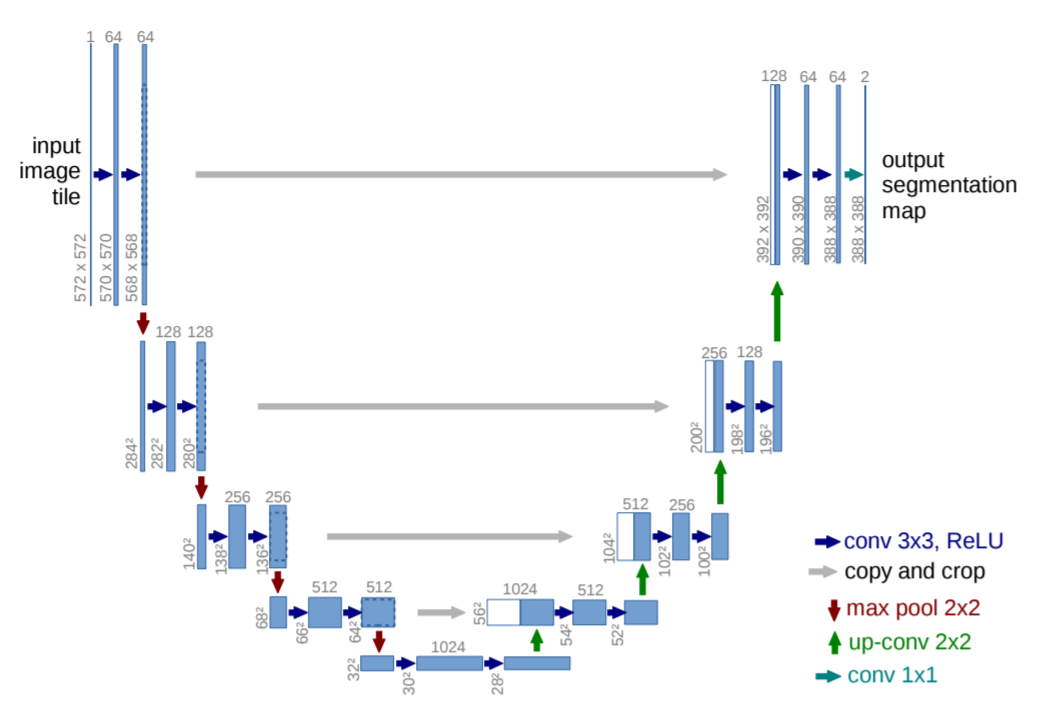
\includegraphics[width=.8\columnwidth]{report/images/UNet.png}
    \caption{
        U-Net example as described in the original paper~\cite{ronneberger2015unet}.
        Each blue box corresponds to a multi-channel feature map; the number of channels is found on top of the box, and the dimensions are at the lower left edge of the box.
        White boxes represent copied feature maps.
        The arrows denote the different operations.
    }
    \label{fig:UNetarchitecture}
\end{figure}

\subsection{Loss}\label{loss}
Our model has to classify each pixel into 2 classes, either the area is available for a rooftop solar panel or not. We try the following three losses:
\begin{itemize}
    \item Binary cross entropy (BCE)
    \item Weighted binary cross entropy (wBCE)
    \item L1 loss
\end{itemize}

The weighted binary cross entropy can be used when there is a significant class imbalance, which is indeed the case here:
most pixels are not available for rooftop solar panels. 
The formula for this loss is:
\begin{equation*}
    %L = \frac{1}{N} \sum_{n=1}^N l_n, \\
    L = \frac{1}{N} \sum_{n=1}^N  [py_n \log(\sigma(x_n))
        + (1-y_n) \log(1-\sigma(x_n))],
    %l_n = - [py_n \log(\sigma(x_n))
        %+ (1-y_n) \log(1-\sigma(x_n))]
\end{equation*}
where $x_n$ and $y_n$ are respectively the output of the model and the true class (0 or 1) for pixel $n$,
and $p$ is the weight given to the positive class. 
Setting $p>1$ increases the recall, whereas $p<1$ increases the precision.
As described in the documentation of PyTorch we set this weight as
% $\frac{\text{\#negative pixels}}{\text{\#positive pixels}}$
$\frac{\mathrm{support}(0)}{\mathrm{support}(1)}$
in the dataset.


\subsection{Training}
We train the model with different parameters and choose the best combination which has the best results on the validation set. We vary the following parameters:

\subsubsection{Optimizer}
We decide to try Adam~\cite{kingma2014adam} and Stochastic Gradient Descent (SGD) to train the U-Net.

\subsubsection{Effect of using noPV images during training}
We try using different amounts of noPV images during training. We think that using too little might make for a model which doesn't generalize well, while using too much might bias the model. We measure the amount of noPV images by considering the percentage of noPV images compared to PV images in the train set. The percentageswe consider are $0\%, 25\% \text{ and } 50\%$.

\subsubsection{Loss}
We use the three losses mentioned in \autoref{loss}. For the weighted cross entropy loss we use a different weight based on the percentage of noPV images we use in the train set. We compute the following weight using the formula from \autoref{loss}.
\begin{center}
    \begin{tabular}{||c | c||} 
        \hline
        Percentage noPV & Weight for wBCE\\ [0.5ex] 
        \hline\hline
        $0\%$ & $5.13$ \\
        \hline
        $25\%$ & $6.46$ \\
        \hline
        $50\%$ & $8.10$ \\
       % [1ex] 
        \hline
    \end{tabular}
\end{center}

\subsubsection{Learning rate scheduling}
We try different constant values of the learning rate of the optimizer. However, small values tend to reach a better minimum of the loss function but very slowly, while big values are faster but don't guarantee a good convergence. We propose to use a learning rate scheduler to combine the best of both. We start training with a larger learning rate and decrease it during training.

\subsection{Tuning threshold on probability after training model} \label{ssec:threshold}
Since the model outputs weights (real numbers in all of $\mathbb{R}$) for each pixel,
we use a sigmoid to transform the weights into numbers in $[0,1]$.
Once this is done, we still need to find the best decision boundary---the threshold probability $\theta$ over which a pixel is decided to be available for PV.
For that we perform a grid-search over thresholds, computing the $F_1$-score over our validation set 
for each threshold.
%Finally, we compute the median $Q_2(\theta)$ for each threshold and find the one that maximizes this.
%Then, we compute order statistics (first, second and third quartiles) and find the threshold that maximizes the following metric:
%\begin{equation} \label{eq:threshold_metric}
%    f(\theta) = Q_2(\theta) - (Q_3(\theta) - Q_1(\theta))
%\end{equation}
%where $Q_i$ is the $i$\textsuperscript{th} quartile.
%Our reasoning is that while the median $F_1$-score
%should be high, we should also prioritize
%values for which we are more certain of the ``true'' $F_1$-score.


As a reminder, the precision of the prediction
corresponds to $\P{\text{Pred}=1 \given \text{Label} = 1}$ while
the recall corresponds to $\P{\text{Label}=1 \given \text{Pred} = 1}$.
As such, both are susceptible to become undefined if
$\#\tl1 = 0$ or $\#\pl1 = 0$, respectively.

Since we must have noPV images in the validation and test sets in order to faithfully represent real-world usage,
these possibilities must be accounted for.
By default, the precision and recall functions we use
can catch these errors and arbitrarily set the value to
0 or to 1.

Setting the value to 0 in case of noPV is not sensible,
because in this case, even if the model perfectly predicts
all pixels as 0, both precision and recall will be set to 0
(hence so will the $F_1$-score).
However, setting the value to 1 also seems suboptimal, because
then we can't make the difference between a model that
perfectly predicted where a PV area was, and a model
that did any prediction on a noPV image.
In both cases, the $F_1$-score is being influenced artificially.

Another solution was then to compute precision and recall
as weighted averages, as is done with multi-class
problems.
In this case, we compute the metrics 
with 1 as the positive class and also with 0 as the
positive class, and then take a weighted average of
the two; the weights are the support of each class.
That way, division-by-zero issues naturally disappear.
Unfortunately, this tended to give a disproportionate
boost to the precision whereas the recall is not as
affected (in fact, it becomes equal to the accuracy).

Finally, we decided that we would be \textbf{concatenating all the images
in the set} and computing each metric just once.
That way, though we lose out on the statistical power
that computing for each image might bring, we are
certain that no undefined behaviour will occur.

\subsection{Testing}
Once the best threshold is found, we use this to produce
the final model; we apply this on our test set and compute
standard classification metrics for each prediction,
using the last method presented in \autoref{ssec:threshold}.

On top of the precision, recall and $F_1$-score we used
to find the best threshold, we also use the
Jaccard loss, or intersection-over-union (IoU) as
it corresponds to the tightness of the overlap between
predicted and true labels.
If our task is used to estimate the total area available
for PV, this tightness is a very relevant metric.


\section{Results}
After selecting appropriate learning rates we choose to train the following models:
\begin{table}
    \begin{center}
        \begin{tabular}{||c | c c c c||}
             \hline
             N\degree & Optimizer & $\%$noPV & Learning rate & Loss \\ \hline\hline
1 & ADAM & $0\% $ & $10^{-3}$ & wBCE \\ \hline
2 & ADAM & $0\% $ & $10^{-4}$ & wBCE \\ \hline
3 & ADAM & $0\% $ & $10^{-3}$ and $10^{-4}$ & wBCE \\ \hline
4 & ADAM & $25\% $ & $10^{-3}$  & wBCE \\ \hline
5 & ADAM & $25\% $ & $10^{-4}$ & wBCE \\ \hline
6 & ADAM & $25\% $ & $10^{-3}$ and $10^{-4}$ & wBCE \\ \hline
7 & ADAM & $50\% $ & $10^{-3}$ & wBCE \\ \hline
8 & ADAM & $50\% $ & $10^{-4}$ & wBCE \\ \hline
9 & ADAM & $50\% $ & $10^{-3}$ and $10^{-4}$ & wBCE \\ \hline
10 & SGD & $0\% $ & $10^{-3}$ & wBCE \\ \hline
11 & SGD & $0\% $ & $10^{-2}$ & wBCE \\ \hline
12 & SGD & $0\% $ & $10^{-2}$ and $10^{-3}$ & wBCE \\ \hline
13 & SGD & $25\% $ & $10^{-3}$ & wBCE \\ \hline
14 & SGD & $25\% $ & $10^{-2}$ & wBCE \\ \hline
15 & SGD & $25\% $ & $10^{-2}$ then $10^{-3}$ & wBCE \\ \hline
16 & SGD & $50\% $ & $10^{-3}$ & wBCE \\ \hline
17 & SGD & $50\% $ & $10^{-2}$ & wBCE \\ \hline
18 & SGD & $50\% $ & $10^{-2}$ and $10^{-3}$ & wBCE \\ \hline
19 & ADAM & $0\% $ & $10^{-3}$ and $10^{-4}$ & BCE \\ \hline
20 & ADAM & $25\% $ & $10^{-3}$ and $10^{-4}$ & BCE \\ \hline
21 & ADAM & $50\% $ & $10^{-3}$ and $10^{-4}$ & BCE \\ \hline
22 & ADAM & $0\% $ & $10^{-3}$ and $10^{-4}$ & L1 \\ \hline
23 & ADAM & $25\% $ & $10^{-3}$ and $10^{-4}$ & L1 \\ \hline
24 & ADAM & $50\% $ & $10^{-3}$ and $10^{-4}$ & L1 \\ \hline
        \end{tabular}
    \end{center}
    \caption{Hyperparameter combinations for the different models we consider. We write two values for the learning rate, when we use learning rate rescheduling. 
    }
    \label{tbl:model_parameters}
\end{table} 



We notice that rescheduling the learning rate during the training only once after 50 epochs gives the best results.
We also notice that when rescheduling, we need to shorten the training to 80 epochs to avoid overfitting,
whereas with a constant learning rate we train for 100 epochs to have the best results before overfitting.

Each model is run on a validation set to perform a grid-search of the best threshold,
and the model is then applied with that threshold to a test set.
Various standard classification metrics are computed and collected in \autoref{tbl:test_results}.

\begin{table}
    \begin{center}
        \begin{tabular}{||c | c c c c||}
             \hline
             Model & Jaccard (IoU) & $F_1$-score & Precision & Recall \\ \hline\hline
 1 & 0.4868 & 0.6548 & 0.5479 & 0.8137 \\ \hline
 2 & 0.5659 & 0.7228 & 0.6542 & 0.8075 \\ \hline
 3 & 0.5159 & 0.6807 & 0.5951 & 0.7949 \\ \hline
 4 & 0.5999 & 0.7499 & 0.7047 & 0.8013 \\ \hline
 5 & 0.4766 & 0.6455 & 0.5629 & 0.7566 \\ \hline
 6 & 0.5921 & 0.7438 & 0.6939 & 0.8015 \\ \hline
 7 & 0.5862 & 0.7391 & 0.7339 & 0.7444 \\ \hline
 8 & 0.5834 & 0.7369 & 0.6716 & 0.8164 \\ \hline
 9 & 0.5781 & 0.7327 & 0.6742 & 0.8022 \\ \hline
10 & 0.2351 & 0.3806 & 0.2745 & 0.6207 \\ \hline
11 & 0.3841 & 0.5550 & 0.4453 & 0.7364 \\ \hline
12 & 0.4703 & 0.6397 & 0.5533 & 0.7581 \\ \hline
13 & 0.3471 & 0.5153 & 0.4583 & 0.5885 \\ \hline
14 & 0.5265 & 0.6898 & 0.6149 & 0.7856 \\ \hline
15 & 0.5685 & 0.7249 & 0.6707 & 0.7887 \\ \hline
16 & 0.4026 & 0.5741 & 0.5190 & 0.6422 \\ \hline
17 & 0.4570 & 0.6273 & 0.5915 & 0.6678 \\ \hline
18 & 0.5493 & 0.7091 & 0.6493 & 0.7810 \\ \hline
19 & 0.5472 & 0.7073 & 0.6550 & 0.7688 \\ \hline
20 & 0.5762 & 0.7311 & 0.6932 & 0.7735 \\ \hline
21 & 0.6223 & 0.7672 & 0.7491 & 0.7862 \\ \hline
22 & 0.5609 & 0.7186 & 0.6919 & 0.7476 \\ \hline
23 & 0.5338 & 0.6961 & 0.6650 & 0.7303 \\ \hline
24 & 0.5243 & 0.6879 & 0.6530 & 0.7268 \\ \hline

        \end{tabular}
    \end{center}
    \caption{Test results for all models, each with its best threshold according to $\arg\max F_1(\theta)$.
    }
    \label{tbl:test_results}
\end{table}

We choose the model 21 as the best model based on the $F_1$-score. We note that basing our choice on the IoU metric would also result in the same chosen method. The train and validation error during training are shown in \autoref{fig:train_validation_errors}. We see that there are some peaks but their frequency and intensity decreases after the rescheduling after 50 epochs. This suggests that using the learning rate scheduling was a good idea. \autoref{fig:precision_recall} shows how we set the threshold for this model.



\begin{figure}
\centering
    \begin{minipage}[b]{.45\columnwidth}
        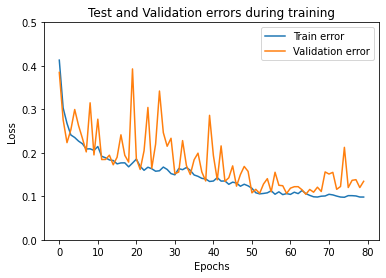
\includegraphics[width=\columnwidth]{report/images/train_validation_errors.png}
        \caption{Train and validation errors during training of the best model (no. 21).}
        \label{fig:train_validation_errors}
    \end{minipage}\quad
    \begin{minipage}[b]{.45\columnwidth}
        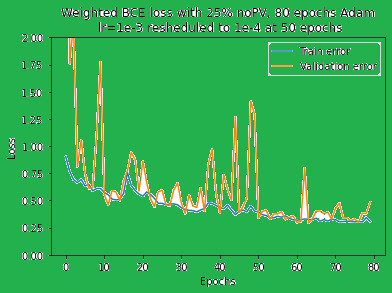
\includegraphics[width=\columnwidth]{report/images/placeholder_precision_recall.png}
        \caption{Precision recall plot placeholder that needs to be changed}
        \label{fig:precision_recall}
    \end{minipage}
\end{figure}

\begin{figure}[tbp]
    \centering
    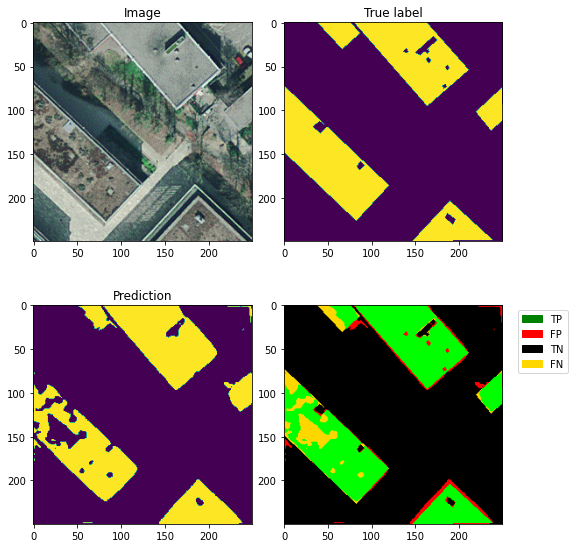
\includegraphics[width=\columnwidth]{report/images/prediction.png}
    \caption{Prediction of the best model (no. 21) on an image from the Test set using a threshold of 0.37.}
    \label{fig:prediction}
\end{figure}

\section{Discussion}
We convince ourselves that this model works well by looking at the predictions it makes. \autoref{fig:prediction} shows the prediction of the model on a test image.
We see that the model recognizes roofs really well and manages to exclude big obstacles and solar panels. However small obstacles on the roof are harder to be recognised by the model and flat ground surfaces similar to roofs can trick the model. From our experience in labelling the data, we can note that the scenarios mentioned above can be hard to label for humans as well.

Here we have used a test set corresponding to the real distribution of PV and noPV images, so that our model stays as general as possible. However if preprocessing can be applied when using this model in order to remove some noPV images, one of the other models might get better performances.

In general, we see that ADAM outperforms SGD.
We observe that using the L1 loss is consistently worse but using the weighted version of BCE does not always give better results. This might be due to the fact that we are basing our predictions on a threshold that we calculate independently of the loss during training. Indeed, the thresholds after using BCE are lower that the ones after using wBCE. 
We also note that training with more noPV images generally gives better results.

Depending on the use case for which this model would be used, it can make more sense to use a different metric to set the threshold value for decisions. If the user wants to minimize the false negative rate, in order to make sure not to underestimate the available area for solar panels, we would suggest to decrease the threshold and increase it in the opposite scenario.

Because we are using a GPU from the lab that is shared with other students running their own experiments we are limited in our computational resources, more fine-tuning of the hyperparameters, especially the learning rate and its scheduler could further increase the performance of our model.

\section{Conclusion}
In this project we propose a model to detect rooftop solar panels in aerial images based on a U-Net. When applied on a test set of images that have not been preprocessed (e.g. removing noPV images), we get a $F_1$-score of $0.77$ and an IoU score of 0.62. 
In our analysis, we fix the decision threshold for this model to $0.37$ but we also give insights on how to change this value depending on the final use of the model.
The U-Net could give better performances with more labelled data, this is not readily available but we give a tool that enables to label new data more easily.

\section*{Acknowledgements}
We would like to thank Prof. Castello and Simon Roquette from his lab for their guidance and valuable advice during this project. We would also like to thank, Riccardo Cadei, Raphael Attias and Shasha Jiang, the members of the other group of the ML course working on the same problem as us with whom we shared our labelled data.
\bibliographystyle{ieeetr}
\bibliography{report}


\end{document}
